\documentclass[a4paper]{article}

%Appearence ----------------------
\usepackage{titling}
\newcommand{\subtitle}[1]{%
  \posttitle{%
    \par\end{center}
    \begin{center}\large#1\end{center}
    \vskip0.5em}%
}
\usepackage{indentfirst}
\usepackage[font={small}]{caption}
\usepackage{geometry}
\geometry{
  margin=2.54cm
}

%Portuguese packages ----------
\usepackage[utf8]{inputenc}
\usepackage[portuguese]{babel}

%Add-ons -----------------------------
\usepackage{booktabs}
\usepackage{graphicx}
\usepackage{amsmath}	
\usepackage{amsfonts}	
\usepackage{tabu}

\title{Relatório de Electromagnetismo I}
\subtitle{Estudo da histerese de um material ferromagnético}
\author{André Duarte, Marcos Gouveia e Sagar Pratapsi}	
\date{3 de Dezembro de 2013}

\begin{document}

\maketitle

\section{Objectivos}
Quando um material ferromagnético é colocado numa zona onde existe um campo $\mathbf{H}$, cria um campo de magnetização, $\mathbf{M}$, sendo que o campo magnético resultante na região é dado por \begin{equation}\label{campos} \mathbf{B}=\mu_0\left( \mathbf{H}+\mathbf{M}\right).\end{equation} Esta magnetização, no entanto, não é apenas uma função do campo externo aplicado, mas também da magnetização pré-existente no material. Existe um efeito de memória a que se chama histerese. 

O objectivo deste trabalho foi obter e analisar a histerese de um material (chave de parafusos) medindo vários valores de $\mathbf{B}$ junto ao mesmo em função do campo $\mathbf{H}$, aplicado por um solenóide. Na Secção 2 explicamos o procedimento utilizado e a razão pela qual o campo $\mathbf{B}$ é uma medida aceitável da magnetização.
\section{Métodos}
Para estudar a curva de histerese, utilizamos uma chave de parafusos, que colocámos no centro de uma bobina. Na bobina fez-se passar uma corrente eléctrica, alimentada por uma fonte de alimentação que permitia variar a intensidade da corrente - medida por um multímetro colocado em série. Assim foi possível criar no centro da bobina um campo magnético, dado aproximadamente por $\mathbf{H}=nI$, sendo $n=1500$ o número de espiras e $I$ a intensidade da corrente. Depois de colocada a chave de parafusos no interior do solenóide, variou-se a intensidade da corrente aplicada e mediu-se o campo $\mathbf{B}$ resultante. Apesar de existirem simultaneamente os campos $\mathbf{H}$ e $\mathbf{M}$ quando a chave se encontra no solenóide, este último tem uma ordem de grandeza consideravelmente superior ao primeiro, pelo que a Equação \ref{campos} pode ser aproximada por $\mathbf{B} \approx \mu_0 \mathbf{M}$. Assim, $\mathbf{B}$ é uma boa estimativa do campo de magnetização.

\subsection{Determinação dos campos $ \mathbf{H}$ e $ \mathbf{B}$}
Para medir os campos magnéticos, usou-se um sensor de Hall (ref.\ SS490A1) que devolve uma diferença de potencial $V$ em função da magnitude do campo detectado, $B$. A curva de calibração que relaciona estes valores é \begin{equation}\label{calibracao}B=320V-800,\end{equation}
com $B$ em Gauss e $V$ em Volt.

O sensor apenas mede o campo \textbf{B} total existente numa região. No entanto, para o nosso objectivo, é necessário determinar o campo \textbf{H} existente independentemente do material ferromagnético. Para isso, dividimos a experência em duas partes:
\begin{enumerate}
\item Medir o campo magnético $B$ sem a chave de parafusos no solenóide, em função da intensidade da corrente $I$ utilizada.  Determinar a expressão para a curva $H(I)$, sabendo que neste caso $H=B/\mu_0$.
\item Medir o campo magnético $B$ com a chave de parafusos no solenóide, em função da corrente $I$ utilizada.
\end{enumerate}

Com base na curva de calibração determinada na primeira parte e nos valores de $I$ obtidos na segunda, podemos determinar o campo $H$ existente quando o ferromagnete se encontra presente. O campo $B$ da segunda parte da experiência, como já vimos, dá-nos a magnetização do material.

Com os resultados obtidos, realizámos um gráfico de $B(H)$ na presença do ferromagnete, para observar a curva de histerese.

\section{Resultados}

\begin{figure*}[htbp]
\centering
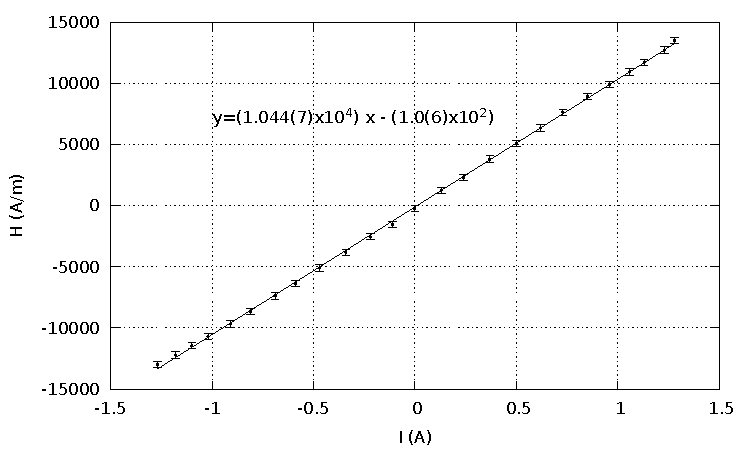
\includegraphics[width=0.7\textwidth]{./Imagens/grafico1.pdf}
\caption{Curva de calibração de $H$ em função de $I$, correspondente a uma recta de equacão $H=(10,44\times 10^3 \pm 68)I-(101\pm 55.05)$}
\end{figure*}

\begin{figure*}[htbp]
\centering
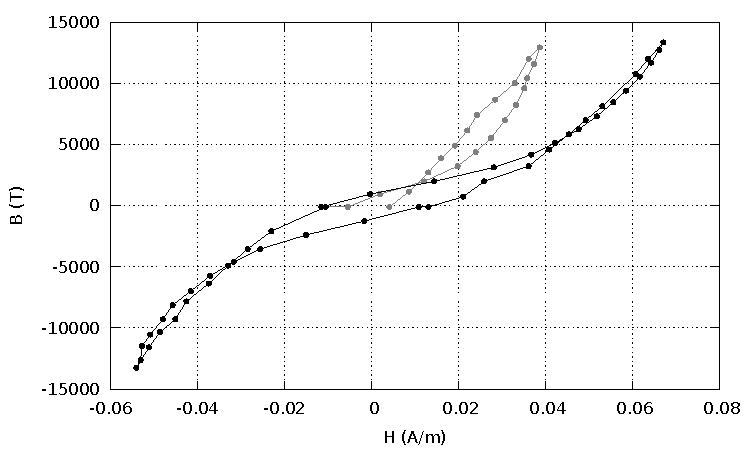
\includegraphics[width=0.7\textwidth]{./Imagens/grafico2.pdf}
\caption{Curva de histerese: campo medido $B$ em função de $H(I)$, determinado pela recta de calibração.}
\end{figure*}

\section{Análise e discussão dos dados}

Na equacão da recta de calibracão do solenóide, podemos interpretar o declive como sendo $n$, o número de espiras por unidade de comprimento do solenóide. Sabendo que o solenóide mede sensívelmene 14,5cm e tem 1500 espiras, obtemos $n=10,34\times 10^3$, o que é coerente com o valor expermiental. O valor da ordenada da origem é bastante pequeno, e pode-se atribuir a erros experimentais.

%Na figura 2 podemos observar o efeito de histerese do material. Em primeiro lugar, vemos um valor nulo de $H$ a corresponder a um valor nulo de $B$, visto que o material não aprezentava magnetiza¢ão remanescente. No entanto, após se atingir o valor máximo de $H$ aplicado, quando realizamos o processo em sentido inverso, o campo $B$ medido para o mesmo valor de $H$ é superior ao medido quando se realizou este processo pela primeira vez. Isto deve-se ao ``efeito de memória'' que resulta da magnetizacao que o material adquiriu durante o primeiro processo. Isto continua a verificar-se, mas em sentido inverso, uma vez aplicando o máximo de corrente negativa e voltando a descer até $H=0$. Repete-se este processo uma vez mais para valores positivos de corrente, verificando-se de novo a histerese no material.

\newpage
\section{Anexos}
\subsection{Dados recolhidos}
\begin{table}[htbp]
\center
\caption{Dados recolhidos para a calibração}
\begin{tabular}{rlrlrlrl}
\hline
\multicolumn{ 2}{c}{I (A)} & \multicolumn{ 2}{c}{V (V)} & \multicolumn{ 2}{c}{B (G)} & \multicolumn{ 2}{c}{H (A/m)} \\ \hline

0.00 & $\pm$ 0.01 & 2.49 & $\pm$ 0.01 & -3.2 & $\pm$ 3.2 & -2.5$\times 10^{2}$ & $\pm 2.5 \times 10^{2}$  \\ 
0.13 & $\pm$ 0.01 & 2.55 & $\pm$ 0.01 & 16.0 & $\pm$ 3.2 & 1.27$\times 10^{3}$ & $\pm 2.5 \times 10^{2}$  \\ 
0.24 & $\pm$ 0.01 & 2.59 & $\pm$ 0.01 & 28.8 & $\pm$ 3.2 & 2.29$\times 10^{3}$ & $\pm 2.5 \times 10^{2}$  \\ 
0.37 & $\pm$ 0.01 & 2.65 & $\pm$ 0.01 & 48.0 & $\pm$ 3.2 & 3.82$\times 10^{3}$ & $\pm 2.5 \times 10^{2}$  \\ 
0.50 & $\pm$ 0.01 & 2.70 & $\pm$ 0.01 & 64.0 & $\pm$ 3.2 & 5.09$\times 10^{3}$ & $\pm 2.5 \times 10^{2}$  \\ 
0.62 & $\pm$ 0.01 & 2.75 & $\pm$ 0.01 & 80.0 & $\pm$ 3.2 & 6.37$\times 10^{3}$ & $\pm 2.5 \times 10^{2}$  \\ 
0.73 & $\pm$ 0.01 & 2.80 & $\pm$ 0.01 & 96.0 & $\pm$ 3.2 & 7.64$\times 10^{3}$ & $\pm 2.5 \times 10^{2}$  \\ 
0.85 & $\pm$ 0.01 & 2.85 & $\pm$ 0.01 & 112.0 & $\pm$ 3.2 & 8.91$\times 10^{3}$ & $\pm 2.5 \times 10^{2}$  \\ 
0.96 & $\pm$ 0.01 & 2.89 & $\pm$ 0.01 & 124.8 & $\pm$ 3.2 & 9.93$\times 10^{3}$ & $\pm 2.5 \times 10^{2}$  \\ 
1.06 & $\pm$ 0.01 & 2.93 & $\pm$ 0.01 & 137.6 & $\pm$ 3.2 & 1.09$\times 10^{4}$ & $\pm 2.5 \times 10^{2}$  \\ 
1.13 & $\pm$ 0.01 & 2.96 & $\pm$ 0.01 & 147.2 & $\pm$ 3.2 & 1.17$\times 10^{4}$ & $\pm 2.5 \times 10^{2}$  \\ 
1.23 & $\pm$ 0.01 & 3.00 & $\pm$ 0.01 & 160.0 & $\pm$ 3.2 & 1.27$\times 10^{4}$ & $\pm 2.5 \times 10^{2}$  \\ 
1.28 & $\pm$ 0.01 & 3.03 & $\pm$ 0.01 & 169.6 & $\pm$ 3.2 & 1.35$\times 10^{4}$ & $\pm 2.5 \times 10^{2}$  \\ 
-0.11 & $\pm$ 0.01 & 2.44 & $\pm$ 0.01 & -19.2 & $\pm$ 3.2 & -1.53$\times 10^{3}$ & $\pm 2.5 \times 10^{2}$  \\ 
-0.22 & $\pm$ 0.01 & 2.40 & $\pm$ 0.01 & -32.0 & $\pm$ 3.2 & -2.55$\times 10^{3}$ & $\pm 2.5 \times 10^{2}$  \\ 
-0.34 & $\pm$ 0.01 & 2.35 & $\pm$ 0.01 & -48.0 & $\pm$ 3.2 & -3.82$\times 10^{3}$ & $\pm 2.5 \times 10^{2}$  \\ 
-0.47 & $\pm$ 0.01 & 2.30 & $\pm$ 0.01 & -64.0 & $\pm$ 3.2 & -5.09$\times 10^{3}$ & $\pm 2.5 \times 10^{2}$  \\ 
-0.59 & $\pm$ 0.01 & 2.25 & $\pm$ 0.01 & -80.0 & $\pm$ 3.2 & -6.37$\times 10^{3}$ & $\pm 2.5 \times 10^{2}$  \\ 
-0.69 & $\pm$ 0.01 & 2.21 & $\pm$ 0.01 & -92.8 & $\pm$ 3.2 & -7.38$\times 10^{3}$ & $\pm 2.5 \times 10^{2}$  \\ 
-0.81 & $\pm$ 0.01 & 2.16 & $\pm$ 0.01 & -108.8 & $\pm$ 3.2 & -8.66$\times 10^{3}$ & $\pm 2.5 \times 10^{2}$  \\ 
-0.91 & $\pm$ 0.01 & 2.12 & $\pm$ 0.01 & -121.6 & $\pm$ 3.2 & -9.68$\times 10^{3}$ & $\pm 2.5 \times 10^{2}$  \\ 
-1.02 & $\pm$ 0.01 & 2.08 & $\pm$ 0.01 & -134.4 & $\pm$ 3.2 & -1.070$\times 10^{4}$ & $\pm 2.5 \times 10^{2}$  \\ 
-1.10 & $\pm$ 0.01 & 2.05 & $\pm$ 0.01 & -144.0 & $\pm$ 3.2 & -1.146$\times 10^{4}$ & $\pm 2.5 \times 10^{2}$  \\ 
-1.18 & $\pm$ 0.01 & 2.02 & $\pm$ 0.01 & -153.6 & $\pm$ 3.2 & -1.222$\times 10^{4}$ & $\pm 2.5 \times 10^{2}$  \\ 
-1.27 & $\pm$ 0.01 & 1.99 & $\pm$ 0.01 & -163.2 & $\pm$ 3.2 & -1.300$\times 10^{4}$ & $\pm 2.5 \times 10^{2}$  \\ 
\hline
\end{tabular}
\label{calibracao}
\end{table}

\begin{table}[htbp]
\center
\caption{Dados recolhidos para a histerese}
\begin{tabular}{rlrlrlrl}
\hline
\multicolumn{ 2}{c}{I (A)} & \multicolumn{ 2}{c}{V (V)} & \multicolumn{ 2}{c}{B (T)} & \multicolumn{ 2}{c}{H (A/m)} \\ \hline
    0     & 0.01 & 2.14 & 0.01 & -0.01152 & 0.00032 & -101.7650355752   & 118.0363192245 \\
    0.1   & 0.01 & 2.49 & 0.01 & -0.00032 & 0.00032 & 942.3409104197    & 118.2302742768 \\
    0.2   & 0.01 & 2.95 & 0.01 & 0.0144   & 0.00032 & 1986.4468564145   & 118.8102396853 \\
    0.31  & 0.01 & 3.38 & 0.01 & 0.02816  & 0.00032 & 3134.9633970089   & 119.8872464539 \\
    0.41  & 0.01 & 3.65 & 0.01 & 0.0368   & 0.00032 & 4179.0693430038   & 121.2554847367 \\
    0.5   & 0.01 & 3.82 & 0.01 & 0.04224  & 0.00032 & 5118.7646943992   & 122.793322879  \\
    0.61  & 0.01 & 3.99 & 0.01 & 0.04768  & 0.00032 & 6267.2812349935   & 125.050888076  \\
    0.71  & 0.01 & 4.12 & 0.01 & 0.05184  & 0.00032 & 7311.3871809884   & 127.4465218123 \\
    0.82  & 0.01 & 4.24 & 0.01 & 0.05568  & 0.00032 & 8459.9037215827   & 130.4371586117 \\
    0.91  & 0.01 & 4.33 & 0.01 & 0.05856  & 0.00032 & 9399.5990729781   & 133.1440916675 \\
    1.02  & 0.01 & 4.43 & 0.01 & 0.06176  & 0.00032 & 10548.1156135725  & 136.7487331145 \\
    1.13  & 0.01 & 4.51 & 0.01 & 0.06432  & 0.00032 & 11696.6321541668  & 140.6555353041 \\
    1.23  & 0.01 & 4.57 & 0.01 & 0.06624  & 0.00032 & 12740.7381001617  & 144.4487866338 \\
    1.29  & 0.01 & 4.6  & 0.01 & 0.0672   & 0.00032 & 13367.2016677586  & 146.827543276  \\
    1.16  & 0.01 & 4.49 & 0.01 & 0.06368  & 0.00032 & 12009.8639379653  & 141.7702297567 \\
    1.04  & 0.01 & 4.4  & 0.01 & 0.0608   & 0.00032 & 10756.9368027714  & 137.4373145051 \\
    0.79  & 0.01 & 4.16 & 0.01 & 0.05312  & 0.00032 & 8146.6719377843   & 129.5859449018 \\
    0.68  & 0.01 & 4.04 & 0.01 & 0.04928  & 0.00032 & 6998.1553971899   & 126.6946141599 \\
    0.57  & 0.01 & 3.92 & 0.01 & 0.04544  & 0.00032 & 5849.6388565956   & 124.1830509327 \\
    0.45  & 0.01 & 3.78 & 0.01 & 0.04096  & 0.00032 & 4596.7117214017   & 121.9037773041 \\
    0.32  & 0.01 & 3.63 & 0.01 & 0.03616  & 0.00032 & 3239.3739916084   & 120.0075900724 \\
    0.2   & 0.01 & 3.31 & 0.01 & 0.02592  & 0.00032 & 1986.4468564145   & 118.8102396853 \\
    0.08  & 0.01 & 3.16 & 0.01 & 0.02112  & 0.00032 & 733.5197212207    & 118.160487134  \\
    0     & 0.01 & 2.91 & 0.01 & 0.01312  & 0.00032 & -101.7650355752   & 118.0363192245 \\
    0     & 0.01 & 2.84 & 0.01 & 0.01088  & 0.00032 & -101.7650355752   & 118.0363192245 \\
    -0.11 & 0.01 & 2.45 & 0.01 & -0.0016  & 0.00032 & -1250.2815761696  & 118.2709644269 \\
    -0.22 & 0.01 & 2.03 & 0.01 & -0.01504 & 0.00032 & -2398.7981167639  & 118.9721233637 \\
    -0.33 & 0.01 & 1.7  & 0.01 & -0.0256  & 0.00032 & -3547.3146573583  & 120.1316277658 \\
    -0.43 & 0.01 & 1.51 & 0.01 & -0.03168 & 0.00032 & -4591.4206033531  & 121.572524634  \\
    -0.54 & 0.01 & 1.34 & 0.01 & -0.03712 & 0.00032 & -5739.9371439475  & 123.5671176227 \\
    -0.66 & 0.01 & 1.2  & 0.01 & -0.0416  & 0.00032 & -6992.8642791413  & 126.2090091493 \\
    -0.77 & 0.01 & 1.07 & 0.01 & -0.04576 & 0.00032 & -8141.3808197357  & 129.0331074013 \\
    -0.88 & 0.01 & 1    & 0.01 & -0.048   & 0.00032 & -9289.8973603301  & 132.2167476594 \\
    -1    & 0.01 & 0.91 & 0.01 & -0.05088 & 0.00032 & -10542.8244955239 & 136.0701385552 \\
    -1.09 & 0.01 & 0.85 & 0.01 & -0.0528  & 0.00032 & -11482.5198469193 & 139.2014824924 \\
    -1.2  & 0.01 & 0.84 & 0.01 & -0.05312 & 0.00032 & -12631.0363875136 & 143.287776815  \\
    -1.26 & 0.01 & 0.81 & 0.01 & -0.05408 & 0.00032 & -13257.4999551106 & 145.6288620201 \\
    -1.1  & 0.01 & 0.9  & 0.01 & -0.0512  & 0.00032 & -11586.9304415188 & 139.5614907344 \\
    -0.98 & 0.01 & 0.98 & 0.01 & -0.04864 & 0.00032 & -10334.0033063249 & 135.4016809807 \\
    -0.88 & 0.01 & 1.09 & 0.01 & -0.04512 & 0.00032 & -9289.8973603301  & 132.2167476594 \\
    -0.74 & 0.01 & 1.17 & 0.01 & -0.04256 & 0.00032 & -7828.1490359372  & 128.226187282  \\
    -0.6  & 0.01 & 1.33 & 0.01 & -0.03744 & 0.00032 & -6366.4007115444  & 124.8289879723 \\
    -0.46 & 0.01 & 1.47 & 0.01 & -0.03296 & 0.00032 & -4904.6523871516  & 122.0746974666 \\
    -0.33 & 0.01 & 1.61 & 0.01 & -0.02848 & 0.00032 & -3547.3146573583  & 120.1316277658 \\
    -0.19 & 0.01 & 1.78 & 0.01 & -0.02304 & 0.00032 & -2085.5663329655  & 118.7350043807 \\
    0     & 0.01 & 2.17 & 0.01 & -0.01056 & 0.00032 & -101.7650355752   & 118.0363192245 \\
    0     & 0.01 & 2.33 & 0.01 & -0.00544 & 0.00032 & -101.7650355752   & 118.0363192245 \\
    0.1   & 0.01 & 2.56 & 0.01 & 0.00192  & 0.00032 & 942.3409104197    & 118.2302742768 \\
    0.2   & 0.01 & 2.88 & 0.01 & 0.01216  & 0.00032 & 1986.4468564145   & 118.8102396853 \\
    0.32  & 0.01 & 3.12 & 0.01 & 0.01984  & 0.00032 & 3239.3739916084   & 120.0075900724 \\
    0.43  & 0.01 & 3.25 & 0.01 & 0.024    & 0.00032 & 4387.8905322027   & 121.572524634  \\
    0.54  & 0.01 & 3.36 & 0.01 & 0.02752  & 0.00032 & 5536.4070727971   & 123.5671176227 \\
    0.68  & 0.01 & 3.46 & 0.01 & 0.03072  & 0.00032 & 6998.1553971899   & 126.6946141599 \\
    0.8   & 0.01 & 3.54 & 0.01 & 0.03328  & 0.00032 & 8251.0825323838   & 129.8667741353 \\
    0.93  & 0.01 & 3.6  & 0.01 & 0.0352   & 0.00032 & 9608.4202621771   & 133.7758779158 \\
    1.01  & 0.01 & 3.62 & 0.01 & 0.03584  & 0.00032 & 10443.705018973   & 136.4081781142 \\
    1.12  & 0.01 & 3.67 & 0.01 & 0.03744  & 0.00032 & 11592.2215595673  & 140.2885353042 \\
    1.25  & 0.01 & 3.71 & 0.01 & 0.03872  & 0.00032 & 12949.5592893607  & 145.233413695  \\
    1.16  & 0.01 & 3.63 & 0.01 & 0.03616  & 0.00032 & 12009.8639379653  & 141.7702297567 \\
    0.97  & 0.01 & 3.53 & 0.01 & 0.03296  & 0.00032 & 10026.062640575   & 135.0713006836 \\
    0.84  & 0.01 & 3.39 & 0.01 & 0.02848  & 0.00032 & 8668.7249107817   & 131.0190508172 \\
    0.72  & 0.01 & 3.26 & 0.01 & 0.02432  & 0.00032 & 7415.7977755879   & 127.7033508344 \\
    0.6   & 0.01 & 3.19 & 0.01 & 0.02208  & 0.00032 & 6162.870640394    & 124.8289879723 \\
    0.48  & 0.01 & 3.1  & 0.01 & 0.0192   & 0.00032 & 4909.9435052002   & 122.4270515394 \\
    0.38  & 0.01 & 3    & 0.01 & 0.016    & 0.00032 & 3865.8375592053   & 120.8068172451 \\
    0.27  & 0.01 & 2.91 & 0.01 & 0.01312  & 0.00032 & 2717.321018611    & 119.4430309036 \\
    0.12  & 0.01 & 2.77 & 0.01 & 0.00864  & 0.00032 & 1151.1620996187   & 118.3155137729 \\
    0     & 0.01 & 2.63 & 0.01 & 0.00416  & 0.00032 & -101.7650355752   & 118.0363192245 \\
\hline
\end{tabular}
\label{histerese}
\end{table}

\newpage
\subsection{Cálculo dos erros associados às medidas}
Na secção 3, as grandezas obtidas foram medidas directamente, pelo que os erros foram estimados tendo em conta o método de medição usado. No entanto, na secção 4, as grandezas foram calculadas a partir das obtidas directamente, pelo que há propagações de erros envolvidas. Esses erros foram calculados pela fórmula de propagação de erros: \begin{equation} \delta f(x_1,x_2,\ldots,x_n)=\sqrt{\sum_{i=1}^{n}\left( \frac{\partial f}{\partial x_i}\delta x_i \right)^2}\end{equation}.

Aqui, $f$ é uma grandeza calculada a partir das grandezas $x_1,x_2,\ldots,x_n$, e $\delta x_i$ são os erros associados às mesmas. Na Tabela 4 apresentamos as equações das grandezas calculadas bem como os respetivos erros.
\renewcommand{\arraystretch}{2.5}
\begin{table}[htbp]
\begin{center}
\caption{Resumo das equações utilizadas para efectuar o cálculo de grandezas relevantes e o respectivo erro, calculado pela fórmula de propagação de erros - equação (4).}
\begin{tabular}{lll}
\textbf{Grandeza} & $f(x_1,x_2,\ldots,x_n)$ & $\delta f(x_1,x_2,\ldots,x_n)$ \\ \hline
\textbf{Área}&$\displaystyle A=\pi\left(\frac{d}{2}\right)^2 $ & $\displaystyle \delta A= \frac{\pi d}{2}\delta d $ \\
\textbf{Área média} &$\displaystyle A_g=\frac{A_i+A_f}{2}$ & $ \displaystyle\delta A_g=\frac{1}{2}\sqrt{\delta A_i^2+\delta A_f^2}$ \\
\textbf{Taxa de fusão} &$\displaystyle R=R_a=\frac{m_f-m_i}{\Delta t}$&$ \displaystyle\delta R=\delta R_a= \sqrt{\left( \frac{\delta m_i}{\Delta t}\right)^2+\left( \frac{m_f}{\Delta t}\right)^2+\left( \frac{m_f-m_i}{\Delta t^2}\delta(\Delta t)\right)^2}$ \\
\textbf{Taxa de fusão efectiva}&$\displaystyle R_0=R-R_a$ & $ \displaystyle \delta R_0= \sqrt{\delta R^2+\delta R_a^2}$ \\
\textbf{Condutividade}&$\displaystyle k=\frac{R_0 L_g h}{A_g \Delta T} $& $ \displaystyle \delta k= k\sqrt{\left(\frac{\delta R_0}{R_0}\right)^2+\left(\frac{\delta h}{h}\right)^2+\left(\frac{\delta A_g}{A_g}\right)^2}$ \\ [2ex] \hline
\end{tabular}
\end{center}
\end{table}

\end{document}